\documentclass[12pt,a4paper]{article}
\usepackage[utf8]{inputenc}
\usepackage[T1]{fontenc}
\usepackage[french]{babel}
\usepackage[width=1.00cm, height=0.00cm, left=1cm ,right=0.5cm, top=3.2cm, bottom=1.00cm]{geometry}
\usepackage[dvipsnames]{xcolor}
\usepackage{hhline, booktabs}
\usepackage{pifont}
\usepackage{xcolor}
\usepackage{amsfonts}
\usepackage[explicit]{titlesec}
\usepackage{amsmath}
\usepackage{mathrsfs}
\usepackage{diagbox}
\usepackage{makecell}
\usepackage{graphicx}
\usepackage{chemfig}
\usepackage{titletoc}
\usepackage{tabularx}
\usepackage[export]{adjustbox}
\usepackage{multirow}
\usepackage{ccicons}
\usepackage{fontawesome}
\usepackage{marginnote}
\usepackage{lastpage}
\usepackage{minitoc}
\usepackage{array}
\usepackage{tikz}
\usepackage{makeidx}
\usepackage{graphicx}
\usepackage{ textcomp }
\usepackage{ mathrsfs }
\usepackage{ifthen}
\usepackage{anyfontsize}
\usepackage{amsmath}
\usepackage{amssymb}
\usepackage{romanbar}
\everymath{\displaystyle}
\usepackage{lipsum}
\usepackage[most]{tcolorbox}
\usepackage{tikz,everypage,amsmath,etoolbox,pifont,lipsum,multicol,colortbl,array}
\pagestyle{empty}
\parindent=0mm
\usetikzlibrary{positioning,shadows.blur,shapes.multipart,shapes.geometric}
\usetikzlibrary{decorations.pathmorphing}
%%%%%%%%%%%%%%%%%%%%%%%%%%%%%%
\usetikzlibrary{calc}
\usetikzlibrary{shapes}
\usetikzlibrary{arrows.meta}
\usepackage{pgfplots}
\tcbuselibrary{theorems,skins}
\pgfplotsset{compat=newest}
\usetikzlibrary{arrows.meta}
\usetikzlibrary{intersections,decorations.text}
\usetikzlibrary{calc}
\usetikzlibrary{babel}
\everymath{\displaystyle}
%%%%%%%%%%%%%%%%%%%%%%%%%%%%%%
\newcounter{numexo}
\setcounter{numexo}{1}
%%%%%%%%%%%%%%%%%%%%%%%%%%%%%%
\usetikzlibrary{shadows,shadows.blur}
\usepackage[adobe-utopia]{mathdesign}
%============================================
\definecolor{myblue3}{RGB}{36, 57, 126}
\definecolor{mygray}{RGB}{112,121,139}
\definecolor{LemonGlacier}{RGB}{253,255,0}
%=================================================
\colorlet{myblue3}{red!75!black}
\newtcolorbox{tcbtwentytwo}[2][]{%
enhanced,
breakable,width=20.7cm,
before skip=00mm,
after skip=0cm,
bottom=0.5cm,
colframe=red!75!black,
colback=white!2,
coltitle=white,
fonttitle=\bfseries,
boxrule=0.2mm,
arc=2mm,
drop midday shadow=red!50!black,
attach boxed title to top left={
xshift=0cm,
yshift*=0mm-\tcboxedtitleheight
},
%varwidth boxed title*=-3cm,
boxed title style={
interior empty,
%interior engine=empty,
frame code={
\path[fill=red!75!black]
([xshift=+0.5cm]frame.north east)[rounded corners=2mm]--(frame.north west)[sharp corners]--(frame.south west) --(frame.south east)to[out=0,in=180]cycle;
\draw[red!75!black]([yshift=-0.5mm]frame.south west)--([yshift=-0.5mm,xshift=+0.4mm]frame.south east)to[out=0,in=180]([yshift=0mm,xshift=+0.58cm]frame.north east);
},
%
},
title=#2,#1}
%%%%%%%
\usepackage{lastpage}
%%%%%
\newtcolorbox{Exercice}[2][]{%
enhanced,
breakable,
before skip=2mm,
after skip=0.2cm,
bottom=0.5cm,
colframe=red!75!black,
colback=white!2,
coltitle=white,
fonttitle=\bfseries,
boxrule=0.2mm,
arc=2mm,
drop midday shadow=red!50!black,
attach boxed title to top left={
xshift=0cm,
yshift*=0mm-\tcboxedtitleheight
},
%varwidth boxed title*=-3cm,
boxed title style={
interior empty,
%interior engine=empty,
frame code={
\path[fill=red!75!black]
([xshift=+0.5cm]frame.north east)[rounded corners=2mm]--(frame.north west)[sharp corners]--(frame.south west) --(frame.south east)to[out=0,in=180]cycle;
\draw[red!75!black]([yshift=-0.5mm]frame.south west)--([yshift=-0.5mm,xshift=+0.4mm]frame.south east)to[out=0,in=180]([yshift=0mm,xshift=+0.58cm]frame.north east);
},
%
},
title=#2,#1}
%%%%%%%%%%%%%
\newcommand{\numexo}{\textbf{Q}$\thenumexo$ \addtocounter{numexo}{1} }
\AddEverypageHook{%
\tikzpicture[remember picture,overlay]
\path
(current page.north west) coordinate (A)
(current page.north east) coordinate (B)
(current page.south east) coordinate (C)
(current page.south west) coordinate (D)
(current page.center) coordinate (E);
\clip[] (A) rectangle(C);
%%%%%%%%%%%%%%%%%%%% Background %%%%%%%%%%%%%%%%%%%%%%%%
%========================================
%\node[inner sep=0pt] at ([shift={(0,-3.5)}]E) {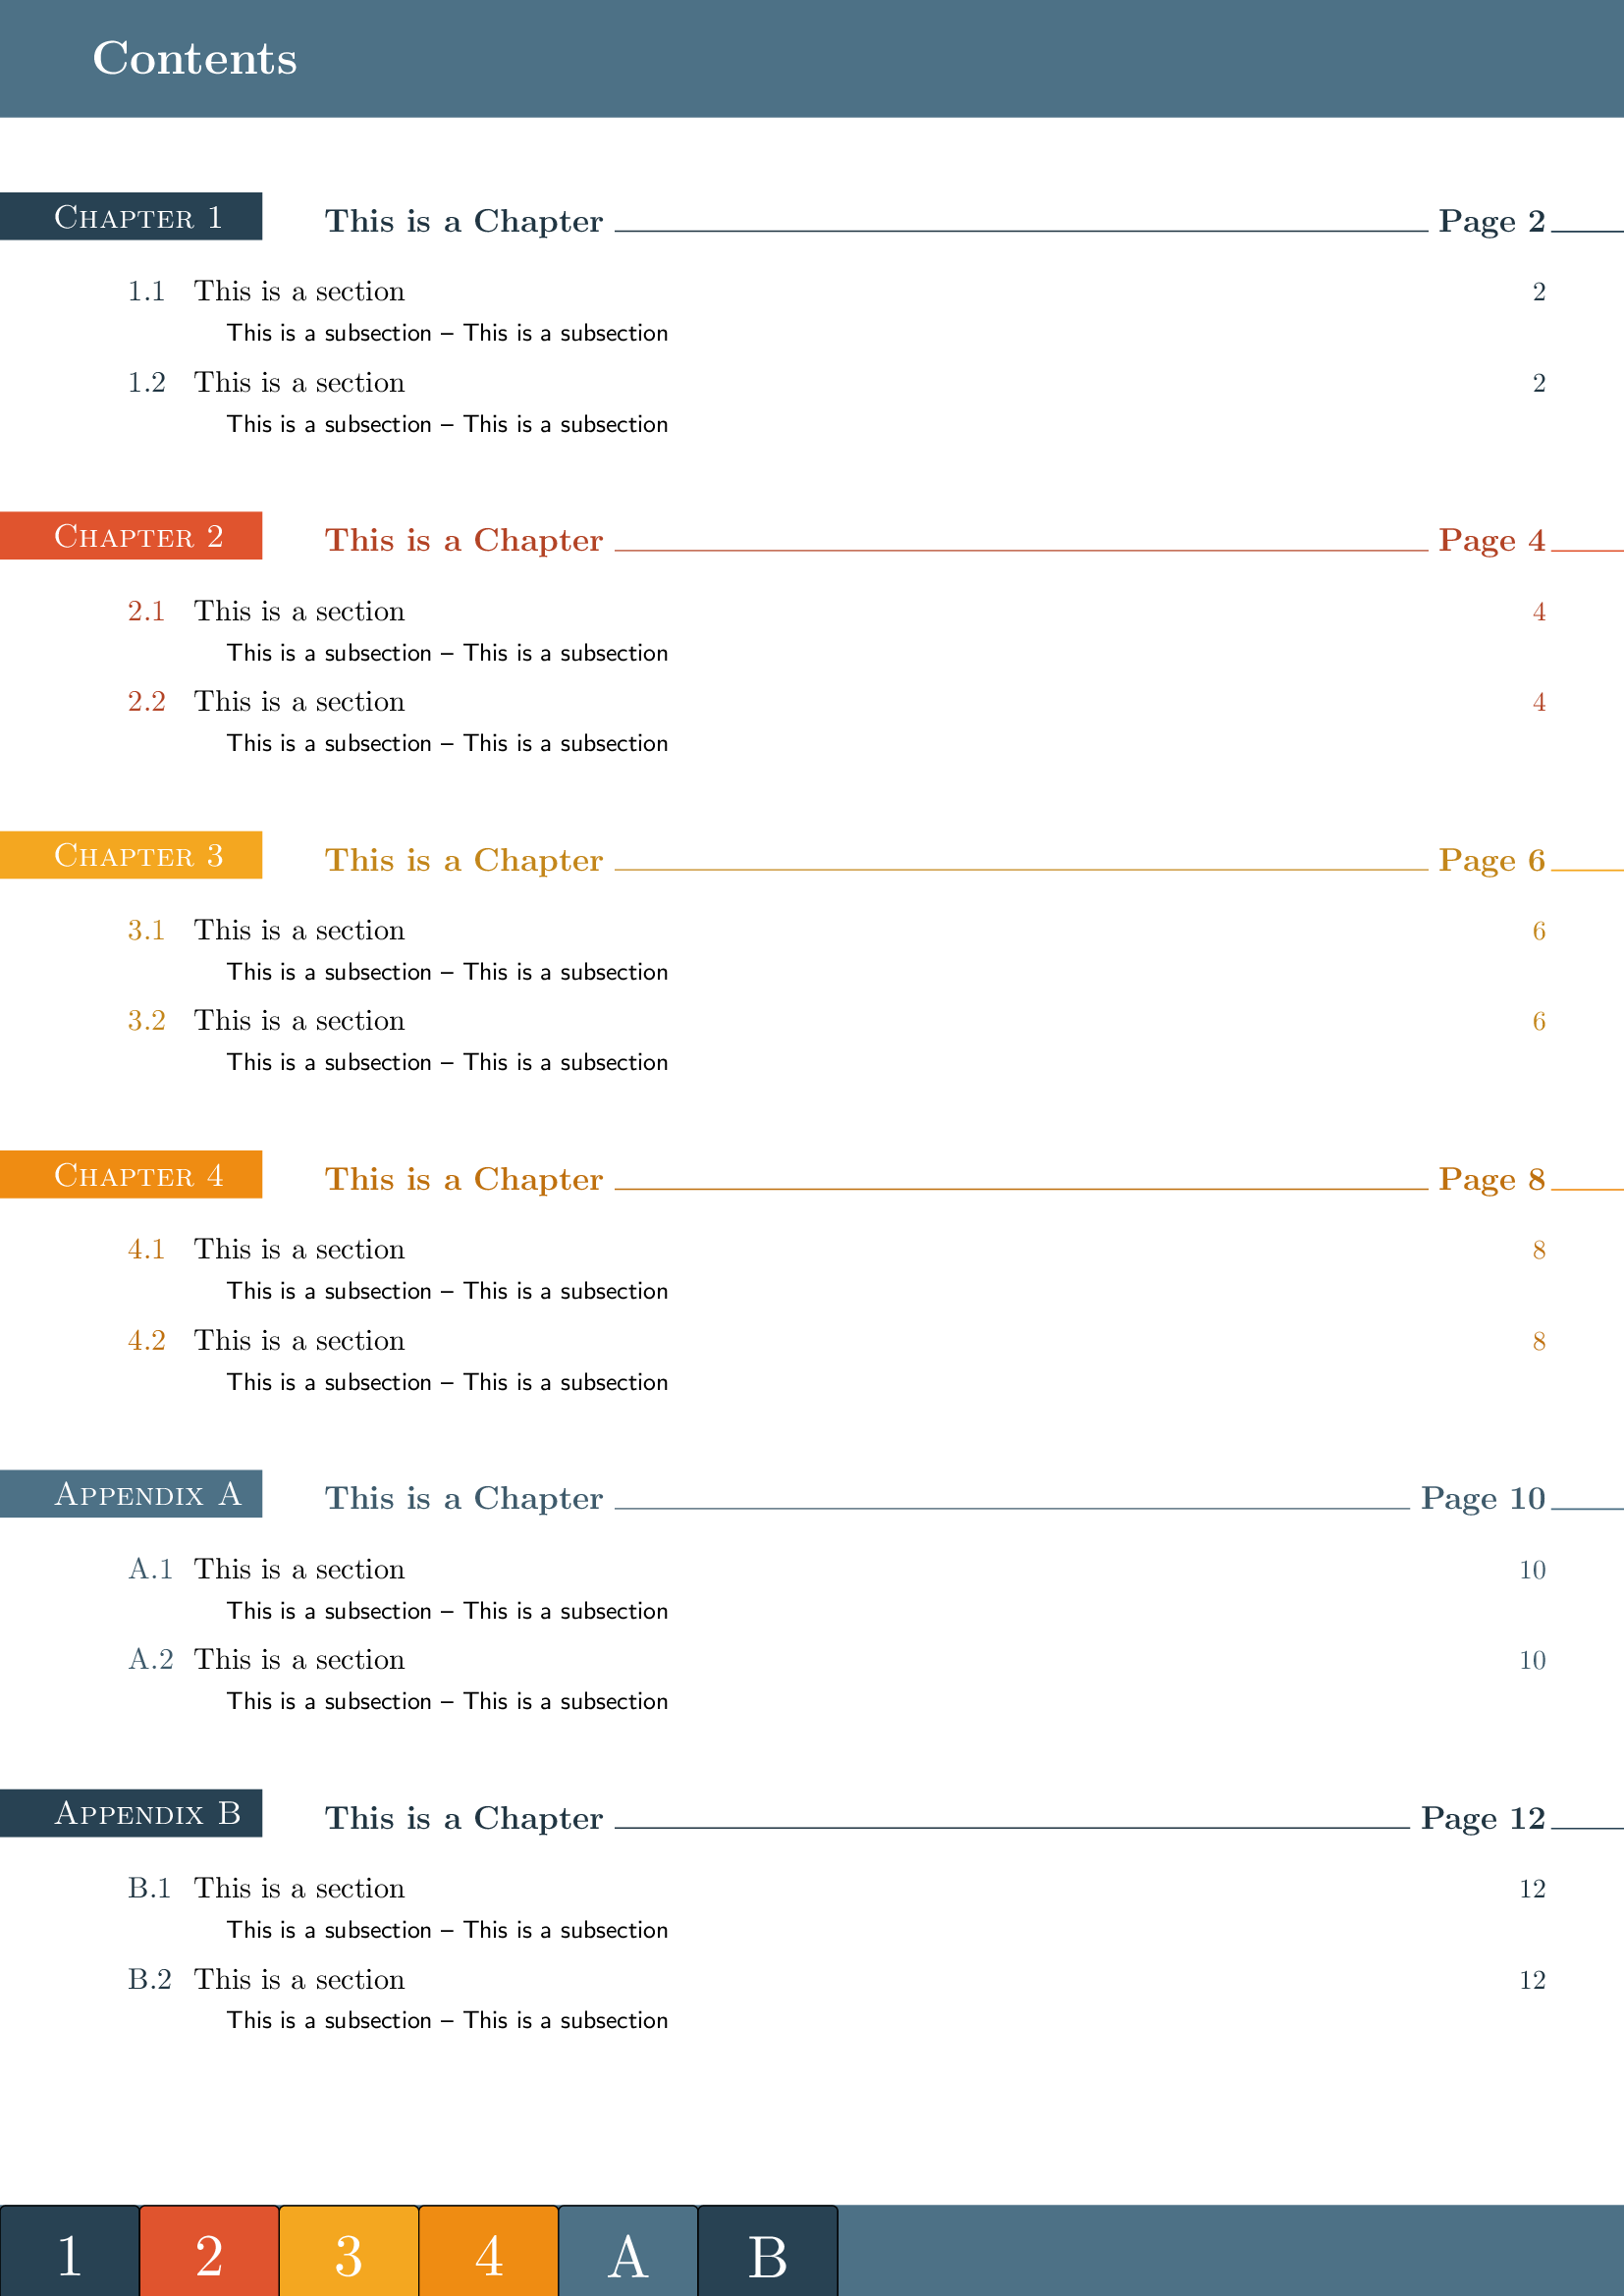
\includegraphics[scale=3]{1.jpg}};
%%%%%%%%%%%%%%ù
%%%%%%%%%
\fill[red!75!black] (current page.south west)-- ([shift={(-3,0)}]current page.south)--++(1,1)-- ([shift={(0,1)}]current page.south west)--cycle;
\fill[LemonGlacier!50] ([shift={(-3,0)}]current page.south)--++(1,1)-- ++(4,0)--++(-1,-1)--cycle;
\fill[red!75!black] (current page.south east)-- ([shift={(1,0)}]current page.south)--++(1,1)-- ([shift={(0,1)}]current page.south east)--cycle;
\draw[cyan,line width=2pt]([shift={(-0,0)}]current page.north east)--([shift={(0,1.0)}]current page.south east);
\draw[myblue3,line width=2pt]([shift={(0,0)}]current page.north west)--([shift={(0,1.0)}]current page.south west);
%========================================================
\node[anchor=west,rotate=90,fill=yellow] at ([shift={(0.5,2)}]current page.south west){\color{red!75!black}\textbf{{\Large Mathématiques}}};
\node[anchor=west,rotate=90,fill=red!75!black] at ([shift={(0.5,9)}]current page.south west){\color{Yellow}\textbf{{  2BAC PC/SVT BIOF  }}};
\node[anchor=west,] at ([shift={(-5,0.5)}]current page.south east){\color{Blue}\textbf{{\large\color{Yellow} \anneee}}};
\node[anchor=west] at ([shift={(1,0.5)}]current page.south west){\color{Yellow}\textbf{{\large \prof}}};
\node[anchor=west] at ([shift={(9.7,0.5)}]current page.south west){\color{red!75!black}\textbf{{\Large \thepage }}};
\node[anchor=west,scale=1,text=Yellow] at ([shift={(0,-1.5)}]current page.north west){\begin{tcbtwentytwo}{\begin{tabular}{p{5cm}p{6cm}}
{ \class}  & { \lycee} \\
{ \prof} & { \duree }\\
\end{tabular} }
\begin{center}
\color{red!75!black} \selectfont\uppercase{ {\Huge \textbf{\sujet}} }
\end{center}
\vspace*{-.5cm}
\end{tcbtwentytwo}};
\node[scale=1,font=\bfseries\color{red!75!black},align=left,] at ([shift={(16,-1)}]A) {Nom d'élève:..............................};
\endtikzpicture}
%%%%%%%%%%%%%%%%%%%%
\newtcbox{\monbox}{enhanced,
frame hidden,boxsep=-1mm,
colback=white,
underlay={%
\fill[red!80,rounded corners=0.5mm] (frame.north west)--([shift={(0mm,0mm)}]frame.north east)--([shift={(0mm,0mm)}]frame.south east) -- ([shift={(0mm,0mm)}]frame.south west) -- cycle;
}
}
\mathversion{bold}
%%%%%%%%%%%%%%%%%%%%%%%%%%%ù
%%%%%%%%%%%%%%%%%%%%%%%%%%%%%%%
%%%%%%%%%%%%%%%%
%%%%%%%%%%%%%
%%%%%%%%%%%%%%%
%%%%%%%%%%%%ù
\newcommand{\prof}{Prof: ................}
\newcommand{\class}{2 BAC PC\& SVT}
\newcommand{\anneee}{2023-2024}
\newcommand{\lycee}{Lycée Qualifiant ...}
\newcommand{\duree}{Durée: 2heures}
\newcommand{\sujet}{Test Diagnostique}
\begin{document}
%\vspace*{1cm}
\begin{Exercice}{Exercice 1 }
{\small
\begin{enumerate}
\item La limite $\lim _{\substack{x \rightarrow 3 \\ x>3}} \frac{x}{3-x}$ égale :
\begin{multicols}{4}
\begin{itemize}
\item[$\square$] $\frac{1}{3}$
\item[$\square$] $ 0 $
\item[$\square$]  $-\infty$
\item[$\square$] $+\infty$
\end{itemize}
\end{multicols}
\item La limite $\lim _{x \rightarrow 0} \frac{\sqrt{1+x^2}-1}{x}$ égale :
\begin{multicols}{4}
\begin{itemize}
\item[$\square$] $+\infty$
\item[$\square$] $ -1 $
\item[$\square$]  $ 0 $
\item[$\square$]  $ \dots $
\end{itemize}
\end{multicols}
\item  La limite $\lim _{x \rightarrow+\infty} \sqrt{x+1}-\sqrt{x}$ égale :
\begin{multicols}{4}
\begin{itemize}
\item[$\square$] 0
\item[$\square$] $+\infty$
\item[$\square$] $ 1 $
\item[$\square$] $-\infty$
\end{itemize}
\end{multicols}
\item  La limite $\lim _{x \rightarrow-\infty} \sqrt{9 x^2+x}-2 x$ égale :
\begin{multicols}{4}
\begin{itemize}
\item[$\square$] $ 2 $
\item[$\square$] $+\infty$
\item[$\square$] $ 1 $
\item[$\square$] $-\infty$
\end{itemize}
\end{multicols}
\item Soit $f$ un fonction définie sur $\mathbb{R}$ tel que $(\forall x \in \mathbb{R}): x^2-x \leq f(x) \leq x^2+x$. On a :
\begin{multicols}{3}
\begin{itemize}
\item[$\square$] $\lim _{x \rightarrow+\infty} f(x)=0 $
\item[$\square$] $ \lim _{x \rightarrow 0} f(x)=+\infty $
\item[$\square$] $ \lim _{x \rightarrow+\infty} f(x)=\dots $
\end{itemize}
\end{multicols}
\end{enumerate}}
\end{Exercice}
\begin{Exercice}{Exercice 2 }
{\small
\begin{enumerate}
\item La limite $\lim _{\substack{x \rightarrow 3 \\ x>3}} \frac{x}{3-x}$ égale :
\begin{multicols}{4}
\begin{itemize}
\item[$\square$] $\frac{1}{3}$
\item[$\square$] $ 0 $
\item[$\square$]  $-\infty$
\item[$\square$] $+\infty$
\end{itemize}
\end{multicols}
\item La limite $\lim _{x \rightarrow 0} \frac{\sqrt{1+x^2}-1}{x}$ égale :
\begin{multicols}{4}
\begin{itemize}
\item[$\square$] $+\infty$
\item[$\square$] $ -1 $
\item[$\square$]  $ 0 $
\item[$\square$]  $ \dots $
\end{itemize}
\end{multicols}
\item  La limite $\lim _{x \rightarrow+\infty} \sqrt{x+1}-\sqrt{x}$ égale :
\begin{multicols}{4}
\begin{itemize}
\item[$\square$] 0
\item[$\square$] $+\infty$
\item[$\square$] $ 1 $
\item[$\square$] $-\infty$
\end{itemize}
\end{multicols}
\item  La limite $\lim _{x \rightarrow-\infty} \sqrt{9 x^2+x}-2 x$ égale :
\begin{multicols}{4}
\begin{itemize}
\item[$\square$] $ 2 $
\item[$\square$] $+\infty$
\item[$\square$] $ 1 $
\item[$\square$] $-\infty$
\end{itemize}
\end{multicols}
\item Soit $f$ un fonction définie sur $\mathbb{R}$ tel que $(\forall x \in \mathbb{R}): x^2-x \leq f(x) \leq x^2+x$. On a :
\begin{multicols}{3}
\begin{itemize}
\item[$\square$] $\lim _{x \rightarrow+\infty} f(x)=0 $
\item[$\square$] $ \lim _{x \rightarrow 0} f(x)=+\infty $
\item[$\square$] $ \lim _{x \rightarrow+\infty} f(x)=\dots $
\end{itemize}
\end{multicols}
\end{enumerate}}
\end{Exercice}
\begin{Exercice}{Exercice 3 }
{\small
\begin{enumerate}
\item La limite $\lim _{\substack{x \rightarrow 3 \\ x>3}} \frac{x}{3-x}$ égale :
\begin{multicols}{4}
\begin{itemize}
\item[$\square$] $\frac{1}{3}$
\item[$\square$] $ 0 $
\item[$\square$]  $-\infty$
\item[$\square$] $+\infty$
\end{itemize}
\end{multicols}
\item La limite $\lim _{x \rightarrow 0} \frac{\sqrt{1+x^2}-1}{x}$ égale :
\begin{multicols}{4}
\begin{itemize}
\item[$\square$] $+\infty$
\item[$\square$] $ -1 $
\item[$\square$]  $ 0 $
\item[$\square$]  $ \dots $
\end{itemize}
\end{multicols}
\item  La limite $\lim _{x \rightarrow+\infty} \sqrt{x+1}-\sqrt{x}$ égale :
\begin{multicols}{4}
\begin{itemize}
\item[$\square$] 0
\item[$\square$] $+\infty$
\item[$\square$] $ 1 $
\item[$\square$] $-\infty$
\end{itemize}
\end{multicols}
\item  La limite $\lim _{x \rightarrow-\infty} \sqrt{9 x^2+x}-2 x$ égale :
\begin{multicols}{4}
\begin{itemize}
\item[$\square$] $ 2 $
\item[$\square$] $+\infty$
\item[$\square$] $ 1 $
\item[$\square$] $-\infty$
\end{itemize}
\end{multicols}
\item Soit $f$ un fonction définie sur $\mathbb{R}$ tel que $(\forall x \in \mathbb{R}): x^2-x \leq f(x) \leq x^2+x$. On a :
\begin{multicols}{3}
\begin{itemize}
\item[$\square$] $\lim _{x \rightarrow+\infty} f(x)=0 $
\item[$\square$] $ \lim _{x \rightarrow 0} f(x)=+\infty $
\item[$\square$] $ \lim _{x \rightarrow+\infty} f(x)=\dots $
\end{itemize}
\end{multicols}
\end{enumerate}}
\end{Exercice}
\end{document}
